%!TEX root = ../thesis.tex
% ******************************* Thesis Appendix B ****************************

\chapter{Clocked Comparators Metastability}
\label{app:comp-metastability}

Comparator metastability is ideally a deterministic process for initial $\Delta V_{out}$ of the cross-coupled inverters that is insufficient for regeneration to reach valid logic levels before the end of the available time $T_{AVL}$. In other words we can determine a $\Delta V_{out}$ range for which the time delay exceed the allotted time for the taking a decision.
% The metastable input voltage range $V_{MET}$ exponentially rises with increasing conversion speeds, i.e. shorter $T_{clk}$.
  Unfortunately, the distribution of the differential input voltage and the noise~\cite{noise_comp_sepke_2009} influence the distribution of the time delay. In consequence the likelihood of metastability is also affected. In this section we analyze both the differential input voltage distribution and the temperature impact on the metastability probability of comparators.

\section{Input signal distribution dependency}
The input probability distribution depends on the shape of the input voltage waveform. In this paper, we assume a Laplace distribution over the full scale input range $V_{FS}$. In this case, the probability of comparator metastability is given by (\ref{eqn:prob_time_delay}) for a Gaussian distribution of the delay at a given $\Delta V_{in}$.

%\begin{equation}
%P(t > T_{AVL}) = \frac{2V_{MET}}{V_{FS}} = \frac{2V_{logic}}{V_{FS}} exp\left(\frac{-T_{AVL}}{\tau_{reg}}\right) \label{eq:prob_met1}
%\end{equation}

%\begin{equation}
%P(t > T_{AVL}) = \frac{2V_{logic}}{A_{P}\times V_{FS}}exp\left(-\frac{T_{AVL}-t_{lin}}{\tau_{reg}}\right) \label{eq:prob_met2}
%\end{equation}
\begin{equation}
P(t > T_{AVL}, \Delta V_{in}) = \frac{1}{2}\left(1-erf\left(\frac{T_{AVL}-\mu_{t}(\Delta V_{in})}{\sqrt{2}\sigma_{t}(\Delta V_{in})}\right)\right)
\label{eqn:prob_time_delay}
\end{equation}

where $\mu_{t}$ is the average of the delay as a random variable, and $\sigma_{t}$ the standard deviation of the delay assuming the law of large numbers applicable. In both the SA and the DT comparator the pre-amplification phase effectively multiplies the input range by a dynamic gain $A_{P}$~\cite{metastability_figueiredo_2013}, and one must subtract $t_{lin}$ obtained in Section~\ref{sec:comp-delay-design} from the $T_{AVL}$.

Considering that $t_{lin}$  itself is a Gaussian distributed random variable~\cite{metastability_figueiredo_2013}, errors on the estimation of the delay and its standard deviation can be translated into an error on the metastability probability. This error on the probability is given by (\ref{eqn:error_prob_met}) based on (\ref{eqn:prob_time_delay}).


\begin{align}
2\varepsilon_{Pmet}& = \int_{-V_{FS}/2}^{+V_{FS}/2}{erf\left(\frac{T_{AVL}-\mu_{t}+\epsilon_{\mu}}{(\sigma_{t}+\epsilon_{\sigma})\sqrt{2}}\right)P(\Delta V_{in})d\Delta V_{in}} \nonumber \\
- &\int_{-V_{FS}/2}^{+V_{FS}/2}{erf\left(\frac{T_{AVL}-\mu_{t}}{\sigma_{t}\sqrt{2}}\right)P(\Delta V_{in})d\Delta V_{in}}
\label{eqn:error_prob_met}
\end{align}

In this equation, $P(\Delta V_{in})$ represents the probability to get a specific value of $\Delta V_{in}$. In our case this is given by a Laplace distribution of probability.

Those general equation can be applied to other system based around a comparator by just changing the equation of the time delay ($\mu_{t}$ and $\sigma_{t}$).

\section{Temperature variation}
To consider the temperature impact on the comparators delay, we have considered that the temperature impact most the carrier mobility in the channel and the threshold voltage of transistors.

Assuming mobility variation take over threshold voltage variation, the probability sensitivity to the temperature of~(\ref{eqn:prob_time_delay}) is defined by equation~(\ref{eqn:prob_time_delay_sensitivity}) where $A_P$ is the amplification factor $\Delta V_{out}(t_{lin}) /\Delta V_{in}$.  

\begin{equation}
\frac{d}{dT}P(t > T_{AVL}, \Delta V_{in}) = 
\frac{\exp\left(-{\left(\frac{T_{AVL}-\mu_{delay}(T, \Delta V_{in})}{\sqrt{2}\sigma_{delay}(\Delta V_{in})}\right)}^2 \right)}{\sqrt{2\pi}\sigma_{delay}(\Delta V_{in})} \frac{d}{dT}t(T, \Delta V_{in})
\label{eqn:prob_time_delay_sensitivity}
\end{equation}
\begin{equation}
\frac{d}{dT}t(T, \Delta V_{in}) \approx 
\frac{3\tau}{2 T_0} \sqrt{\frac{T}{T_0}}\left(\log\left(A_P \frac{V_{logic}}{\Delta V_{out}(t_{lin})} {\left(\frac{T}{T_0}\right)}^\frac{3}{2}\right)+1\right)
\label{eqn:time_delay_sensitivity}
\end{equation}

By being strictly positive, the increasing of temperature always inflates probability to be metastable. In consequence, the temperature will move the probability of metastability towards greater $T_{AVL}$.
%Other metastability analysis consider the noise in the evolution of the output voltages at the metastable region. Though it was acknowledged
%that noise prevents the comparator from staying indefinitely at the metastable point.

\section{Metastability of synchronizers}
In ADCs\@, the comparator is most of the time followed by synchronizers to reduce the likelihood of logic errors propagating past the comparator. We chose to add digital flip-flops (DFF) to act as synchronizers, as show in the \figurename~\ref{fig:metastable_rng}. The clock CLK is defined by his period $T_{CLK}$ whose duty cycle is 50 \%.
%These will capture the logic signals coming out of the inverters added to buffer the cross-coupled latch outputs.

\begin{figure}[htp]
\centering
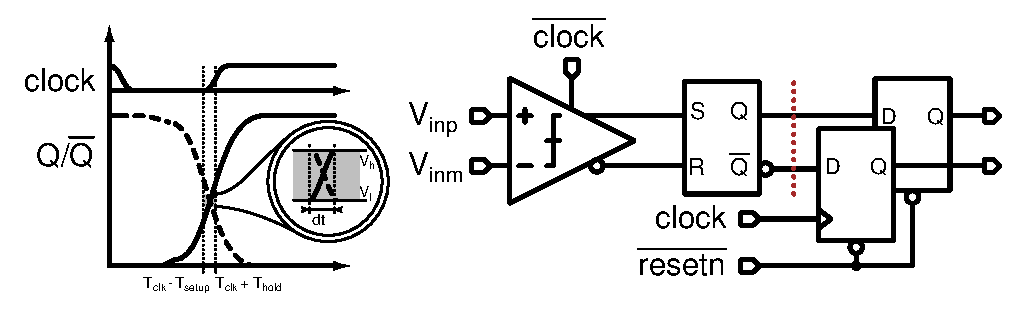
\includegraphics[width=\textwidth]{Appendix3/Figs/comp-metastability-window.ps}
\caption{Metastability input range and test circuit}
\label{fig:metastable_rng}
\end{figure}

Comparator metastability may engender the violation of the set-up and hold times of the DFF\@. In other words, the DFF clock transition may happen too close to the region where the DFF input is between $V_{l}$ and $V_{h}$: the voltage metastable window. Assuming the independence of the probability to be in the forbidden voltage range and the probability to have a transition in the forbidden time span, the probability to be in this generating zone is defined by (\ref{eqn:prob_met_zone_vin}).

\begin{align}
P(Metastability Zone, \Delta V_{in}) &=
P\left(t \in \left[\frac{T_{clk}}{2} \pm \myatop{T_{hold}}{T_{setup}} \right], \Delta V_{in}\right) \nonumber \\
&\times P(V_{out} \in [V_l, V_h])
\label{eqn:prob_met_zone_vin}
\end{align}

% The time spent in the forbidden input voltage range is given by (\ref{eqn:forbidden_voltage_time}) where $\tau$ is the regeneration time constant.

%\begin{equation}
%dt = \tau \ln (V_h/V_l)
%\label{eqn:forbidden_voltage_time}
%\end{equation}

For the sake of simplicity, only the regeneration time is considered since the linear time of comparator can be subtracted to $T_{clk}/2$. And its variation is far less. Hence, the probability to be in the forbidden voltage range at any time is given by equation~(\ref{eqn:prob_forbidden_voltage}) where $\tau_{reg}$ is the regeneration time constant. This probability depends from the temperature due to $V_{out}(t_{lin})$.
\vspace{10pt}
\begin{equation}
P(V_{out} \in [V_l, V_h]) \approx \frac{\tau_{reg}\ln(V_h/V_l)}{\tau_{reg}\ln(V_{logic}/ V_{out}(t_{lin}))}
\label{eqn:prob_forbidden_voltage}
\end{equation}

And, the probability to be in the forbidden time span is easily calculable %by (\ref{eqn:prob_forbidden_time_span})
with the cumulative probability function of the comparator's delay given by the equation (\ref{eqn:prob_time_delay})\cite{metastability_figueiredo_2013}.

%\begin{multline}
%P(t \in [T_{clk}-T_{setup}, T_{clk}+T_{hold}], \Delta V_{in}) = \\
%P(t < T_{clk}+T_{hold}, \Delta V_{in})
%\\ - P(t < T_{clk}-T_{setup}, \Delta V_{in})
%\label{eqn:prob_forbidden_time_span}
%\end{multline}

%Having calculated the mean and the standard deviation of the delay, the probability of $P(t < T_{AVL})$ is given by Equation (\ref{eqn:prob_time_delay})  \cite{metastability_figueiredo_2013}.

Therefore, the probability to be in the metastability generating zone is defined by (\ref{eqn:prob_met_zone}) considering any differential input voltage distribution.

%\begin{multline}
%P(Metastability Zone) = \\
%\frac{1}{V_{FS}} \int_{-V_{FS}/2}^{+V_{FS}/2}{P(Metastability Zone, \Delta V_{in})d\Delta V_{in}} \label{eqn:prob_met_zone}
%\end{multline}
\vspace{-6pt}
\begin{equation}
P(Metastability Zone) = \int_{-V_{FS}/2}^{+V_{FS}/2}{P(Metastability Zone, \Delta V_{in})P(\Delta V_{in})d\Delta V_{in}} \label{eqn:prob_met_zone}
\end{equation}



%And if the delay is beyond the $T_{AVL}$ the probability variation is decreasing since the comparator is already in a metastable state.

In order to compare the SA and the DT comparators, all circuits have been simulated in 0.18-$\mu m$ CMOS technology with $V_{DD} = 1.8 V$. The comparators were designed for offset standard variation of 3 mV at the input common mode voltage of 0.9 V. For the following results, the test setup is depicted by the \figurename~\ref{fig:metastable_rng}. The DFF time constraints are taken to be $t_{setup} = 135 ps$ and $t_{hold} = 70 ps$ while the metastability input range is less than 1 $\mu V$ around 794 mV and varies with the temperature.

%
%Based on the model results, the metastability probability is maximized at the temperature of 175 \degree C.

%%%%%%% do not add this part since it explained only 12 ps about 70 ps and var(t_reg) is preferable %%%%%%%%%%%%
%The linear time variance for the Strong-Arm latch is given by (\ref{eqn:sa_var_tlin}) assuming that the capacitance variation is negligible compared to process variation of the current and the threshold voltage. Furthermore, it is assumed that the correlation of the variation $\mu_X$ and $\Delta_X$ represents respectively the mean and the variation of the random variable $X$.

%\begin{equation}
%\sigma_{t_{lin}}^2 = \left(\frac{\mu_{V_{thp}}(C_{load}+C_p)}{\mu_{I_{M2,M3}}}\right)^2 Var\left(\frac{\Delta_{V_{thp}}}{\mu_{V_{thp}}}+\frac{\Delta_{I_{M2,M3}}}{\mu_{I_{M2,M3}}}\right)\label{eqn:sa_var_tlin}
%\end{equation}

%The one of the Double Tail is roughly given by () with the same assumption than did for the Strong-Arm latch and by neglecting the product of $\Delta X_i/\mu_{X_i}$ and with the assumption of $\sqrt{\xi}$ follows a half normal law.

%\begin{equation}
%\end{equation}

\section{process and temperature variation on the metastability}
The \figurename~\ref{fig:prob_met_zone_temp} depicts the probability for the DT and the SA latches, to enter the metastable zone of DFFs at the clock falling edge. As expected, increasing the temperature decreases the regeneration time constant, and the pre-amplification gain. In turn, the Probability Density Function (PDF) is shifted to lower clock frequencies as explained by the equation (\ref{eqn:prob_time_delay_sensitivity}). This shift is not linear with the temperature but varies according to the variation of the mobility in the CMOS cross-coupled inverters. Based on (\ref{eqn:time_delay_sensitivity}) the estimated $\Delta T_{clk}/2\tau_{reg}$ is 3.3 while the simulation results provide a $\Delta T_{clk}/2\tau_{reg}$ of 3 from $-50 \degree C$ to $+175 \degree C$ for both comparators. 
%As expected a clock frequency delimits horizontally the probability to generate metastability as the comparators delay tends ever closer to $T_{clk}-T_{setup}$. This limit corresponds to a clock period close to the minimal time delay of comparators.
%Moreover, the probability to enter the metastability window of the next component admits a maximum range with the increasing clock frequency and then the probability tends toward zero for very high frequencies. This can be explained by comparators' delay that is much larger than $T_{clk}+T_{hold}$ for any differential input voltage. Increasing the temperature, the lower frequency bound varies less than the maximum probability range. Increasing the temperature, those peaks are placed at frequencies ever closer from this limit. The rate of approaching the lower limit is mainly defined by the variation of the mobility of transistors in the CMOS cross-coupled inverters.
\begin{figure}[htp]
	\centering
	\hspace{0.1cm}
	\begin{subfigure}[b]{0.48\textwidth}
		% Title: glps_renderer figure
% Creator: GL2PS 1.3.9, (C) 1999-2015 C. Geuzaine
% For: Octave
% CreationDate: Fri Oct 28 13:32:32 2016
\setlength{\unitlength}{0.0033\linewidth}
\begin{picture}(0,0)
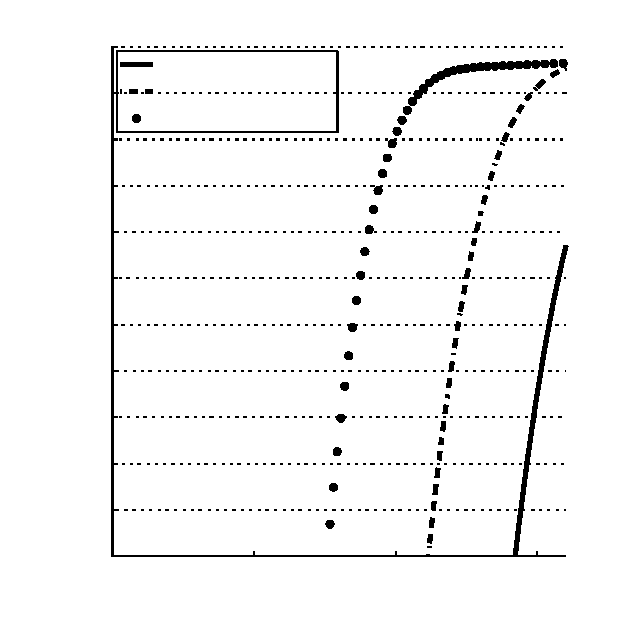
\includegraphics[width=\linewidth]{Appendix3/Figs/DTL_prob_met_zone_temp-inc}
\end{picture}%
\begin{picture}(300,300)(0,0)
\fontsize{8}{0}
\selectfont\put(-7.0039,155.246){\rotatebox{90}{\makebox(0,0)[b]{\textcolor[rgb]{0,0,0}{{P(Met. Zone)}}}}}
\selectfont\put(162.746,10.9883){\makebox(0,0)[t]{\textcolor[rgb]{0,0,0}{{Frequency [MHz]}}}}
\selectfont\put(49.0039,277.492){\makebox(0,0)[r]{\textcolor[rgb]{0,0,0}{{1e-07}}}}
%\selectfont\put(49.0039,255.266){\makebox(0,0)[r]{\textcolor[rgb]{0,0,0}{{1e-08}}}}
\selectfont\put(49.0039,233.039){\makebox(0,0)[r]{\textcolor[rgb]{0,0,0}{{1e-09}}}}
%\selectfont\put(49.0039,210.813){\makebox(0,0)[r]{\textcolor[rgb]{0,0,0}{{1e-10}}}}
\selectfont\put(49.0039,188.586){\makebox(0,0)[r]{\textcolor[rgb]{0,0,0}{{1e-11}}}}
%\selectfont\put(49.0039,166.359){\makebox(0,0)[r]{\textcolor[rgb]{0,0,0}{{1e-12}}}}
\selectfont\put(49.0039,144.133){\makebox(0,0)[r]{\textcolor[rgb]{0,0,0}{{1e-13}}}}
%\selectfont\put(49.0039,121.906){\makebox(0,0)[r]{\textcolor[rgb]{0,0,0}{{1e-14}}}}
\selectfont\put(49.0039,99.6797){\makebox(0,0)[r]{\textcolor[rgb]{0,0,0}{{1e-15}}}}
%\selectfont\put(49.0039,77.4531){\makebox(0,0)[r]{\textcolor[rgb]{0,0,0}{{1e-16}}}}
\selectfont\put(49.0039,55.2266){\makebox(0,0)[r]{\textcolor[rgb]{0,0,0}{{1e-17}}}}
%\selectfont\put(49.0039,33){\makebox(0,0)[r]{\textcolor[rgb]{0,0,0}{{1e-18}}}}
\selectfont\put(257.902,27.9883){\makebox(0,0)[t]{\textcolor[rgb]{0,0,0}{{200}}}}
\selectfont\put(189.934,27.9883){\makebox(0,0)[t]{\textcolor[rgb]{0,0,0}{{150}}}}
\selectfont\put(121.961,27.9883){\makebox(0,0)[t]{\textcolor[rgb]{0,0,0}{{100}}}}
\fontsize{7}{0}
\selectfont\put(74.9961,270.992){\makebox(0,0)[l]{\textcolor[rgb]{0,0,0}{{$-50 \degree C$}}}}
\selectfont\put(74.9961,257.992){\makebox(0,0)[l]{\textcolor[rgb]{0,0,0}{{$+25 \degree C$}}}}
\selectfont\put(74.9961,245.992){\makebox(0,0)[l]{\textcolor[rgb]{0,0,0}{{$+175 \degree C$}}}}
\fontsize{8}{0}
\selectfont\put(53.9922,27.9883){\makebox(0,0)[t]{\textcolor[rgb]{0,0,0}{{50}}}}
\end{picture}

		\subcaption{Double Tail}
		\label{fig:dtl_prob_met_zone_temp}
	\end{subfigure}
	\hspace{0.25cm}
	\begin{subfigure}[b]{0.48\textwidth}
		% Title: glps_renderer figure
% Creator: GL2PS 1.3.9, (C) 1999-2015 C. Geuzaine
% For: Octave
% CreationDate: Fri Oct 28 13:32:32 2016
\setlength{\unitlength}{0.0033\linewidth}
\begin{picture}(0,0)
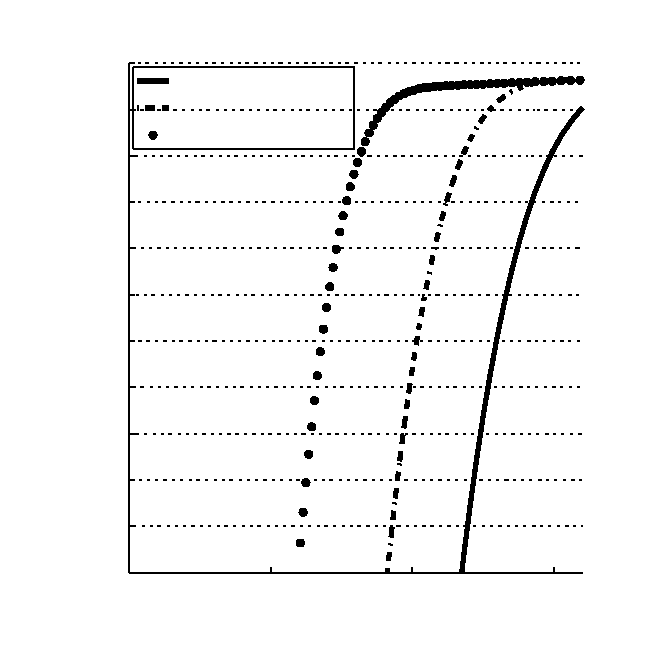
\includegraphics[width=\linewidth]{Appendix3/Figs/SA_prob_met_zone_temp-inc}
\end{picture}%
\begin{picture}(300,300)(0,0)
\fontsize{8}{0}
\selectfont\put(-7.0039,155.246){\rotatebox{90}{\makebox(0,0)[b]{\textcolor[rgb]{0,0,0}{{P(Met. Zone)}}}}}
\selectfont\put(162.746,10.9883){\makebox(0,0)[t]{\textcolor[rgb]{0,0,0}{{Frequency [MHz]}}}}
\selectfont\put(49.0039,277.492){\makebox(0,0)[r]{\textcolor[rgb]{0,0,0}{{1e-07}}}}
%\selectfont\put(49.0039,255.266){\makebox(0,0)[r]{\textcolor[rgb]{0,0,0}{{1e-08}}}}
\selectfont\put(49.0039,233.039){\makebox(0,0)[r]{\textcolor[rgb]{0,0,0}{{1e-09}}}}
%\selectfont\put(49.0039,210.813){\makebox(0,0)[r]{\textcolor[rgb]{0,0,0}{{1e-10}}}}
\selectfont\put(49.0039,188.586){\makebox(0,0)[r]{\textcolor[rgb]{0,0,0}{{1e-11}}}}
%\selectfont\put(49.0039,166.359){\makebox(0,0)[r]{\textcolor[rgb]{0,0,0}{{1e-12}}}}
\selectfont\put(49.0039,144.133){\makebox(0,0)[r]{\textcolor[rgb]{0,0,0}{{1e-13}}}}
%\selectfont\put(49.0039,121.906){\makebox(0,0)[r]{\textcolor[rgb]{0,0,0}{{1e-14}}}}
\selectfont\put(49.0039,99.6797){\makebox(0,0)[r]{\textcolor[rgb]{0,0,0}{{1e-15}}}}
%\selectfont\put(49.0039,77.4531){\makebox(0,0)[r]{\textcolor[rgb]{0,0,0}{{1e-16}}}}
\selectfont\put(49.0039,55.2266){\makebox(0,0)[r]{\textcolor[rgb]{0,0,0}{{1e-17}}}}
%\selectfont\put(49.0039,33){\makebox(0,0)[r]{\textcolor[rgb]{0,0,0}{{1e-18}}}}
\selectfont\put(257.902,27.9883){\makebox(0,0)[t]{\textcolor[rgb]{0,0,0}{{200}}}}
\selectfont\put(189.934,27.9883){\makebox(0,0)[t]{\textcolor[rgb]{0,0,0}{{150}}}}
\selectfont\put(121.961,27.9883){\makebox(0,0)[t]{\textcolor[rgb]{0,0,0}{{100}}}}
\fontsize{7}{0}
\selectfont\put(74.9961,270.992){\makebox(0,0)[l]{\textcolor[rgb]{0,0,0}{{$-50 \degree C$}}}}
\selectfont\put(74.9961,257.992){\makebox(0,0)[l]{\textcolor[rgb]{0,0,0}{{$+25 \degree C$}}}}
\selectfont\put(74.9961,245.992){\makebox(0,0)[l]{\textcolor[rgb]{0,0,0}{{$+175 \degree C$}}}}
\fontsize{8}{0}
\selectfont\put(53.9922,27.9883){\makebox(0,0)[t]{\textcolor[rgb]{0,0,0}{{50}}}}
\end{picture}

		\subcaption{Strong ARM}
		\label{fig:SA_prob_met_zone_temp}
	\end{subfigure}
	\caption{P(Metastability) of DFFs for -50$\degree C$, +25$\degree C$, +175$\degree C$, $\Delta V_{in} \in \pm 450 mV$}
	\label{fig:prob_met_zone_temp}
\end{figure}
Therefore, the temperature variation to generate metastability is more linked to the fabrication process than to the topology.

As a proof the derivative of the probability of metastability  with respect to frequency versus the advancement in the rising of probability is represented in the Figure \ref{fig:slop_deriv_sa_dt_temp}.

\begin{figure}[htp]
 \centering
 \begin{subfigure}[b]{0.48\textwidth}
  % Title: glps_renderer figure
% Creator: GL2PS 1.3.9, (C) 1999-2015 C. Geuzaine
% For: Octave
% CreationDate: Wed Feb 22 11:44:40 2017
\setlength{\unitlength}{0.0033\linewidth}
\begin{picture}(0,0)
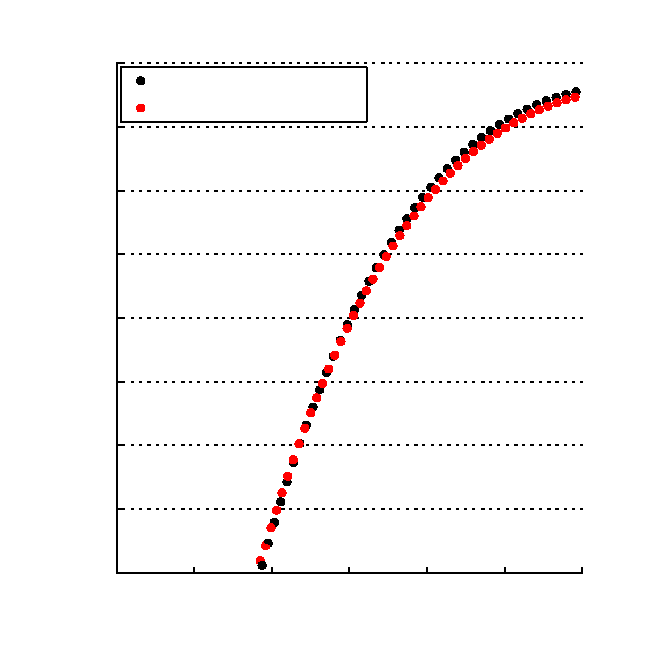
\includegraphics[width=\linewidth]{Appendix3/Figs/sa_dtl_slope_comp_25-inc}
\end{picture}%
\begin{picture}(300,300)(0,0)
\fontsize{8}{0}
\selectfont\put(271.496,27.9883){\makebox(0,0)[t]{\textcolor[rgb]{0,0,0}{{1}}}}
\selectfont\put(43.0117,277.492){\makebox(0,0)[r]{\textcolor[rgb]{0,0,0}{{1e-14}}}}
\selectfont\put(43.0117,246.93){\makebox(0,0)[r]{\textcolor[rgb]{0,0,0}{{1e-16}}}}
\selectfont\put(43.0117,216.371){\makebox(0,0)[r]{\textcolor[rgb]{0,0,0}{{1e-18}}}}
\selectfont\put(43.0117,185.809){\makebox(0,0)[r]{\textcolor[rgb]{0,0,0}{{1e-20}}}}
\selectfont\put(43.0117,155.246){\makebox(0,0)[r]{\textcolor[rgb]{0,0,0}{{1e-22}}}}
\selectfont\put(43.0117,124.684){\makebox(0,0)[r]{\textcolor[rgb]{0,0,0}{{1e-24}}}}
\selectfont\put(43.0117,94.1211){\makebox(0,0)[r]{\textcolor[rgb]{0,0,0}{{1e-26}}}}
\selectfont\put(43.0117,63.5625){\makebox(0,0)[r]{\textcolor[rgb]{0,0,0}{{1e-28}}}}
\selectfont\put(43.0117,33){\makebox(0,0)[r]{\textcolor[rgb]{0,0,0}{{1e-30}}}}
\selectfont\put(159.75,8.9883){\makebox(0,0)[t]{\textcolor[rgb]{0,0,0}{{Slope progression}}}}
\selectfont\put(-10.0117,155.246){\rotatebox{90}{\makebox(0,0)[b]{\textcolor[rgb]{0,0,0}{{dP(Met.)/dF [1/Hz]}}}}}
\selectfont\put(234.246,27.9883){\makebox(0,0)[t]{\textcolor[rgb]{0,0,0}{{0.95}}}}
\selectfont\put(196.996,27.9883){\makebox(0,0)[t]{\textcolor[rgb]{0,0,0}{{0.9}}}}
\selectfont\put(159.75,27.9883){\makebox(0,0)[t]{\textcolor[rgb]{0,0,0}{{0.85}}}}
\selectfont\put(122.5,27.9883){\makebox(0,0)[t]{\textcolor[rgb]{0,0,0}{{0.8}}}}
\selectfont\put(85.25,27.9883){\makebox(0,0)[t]{\textcolor[rgb]{0,0,0}{{0.75}}}}
\selectfont\put(48,27.9883){\makebox(0,0)[t]{\textcolor[rgb]{0,0,0}{{0.7}}}}
\fontsize{7}{0}
\selectfont\put(68.9961,268.992){\makebox(0,0)[l]{\textcolor[rgb]{0,0,0}{{Double Tail}}}}
\selectfont\put(68.9961,255.992){\makebox(0,0)[l]{\textcolor[rgb]{0,0,0}{{Strong Arm}}}}
\end{picture}

   \subcaption{DT/SA comparison}
   \label{fig:sa_dtl_slope_temp}
 \end{subfigure}
 \begin{subfigure}[b]{0.48\textwidth}
  % Title: glps_renderer figure
% Creator: GL2PS 1.3.9, (C) 1999-2015 C. Geuzaine
% For: Octave
% CreationDate: Wed Feb 22 11:50:58 2017
\setlength{\unitlength}{0.0033\linewidth}
\begin{picture}(0,0)
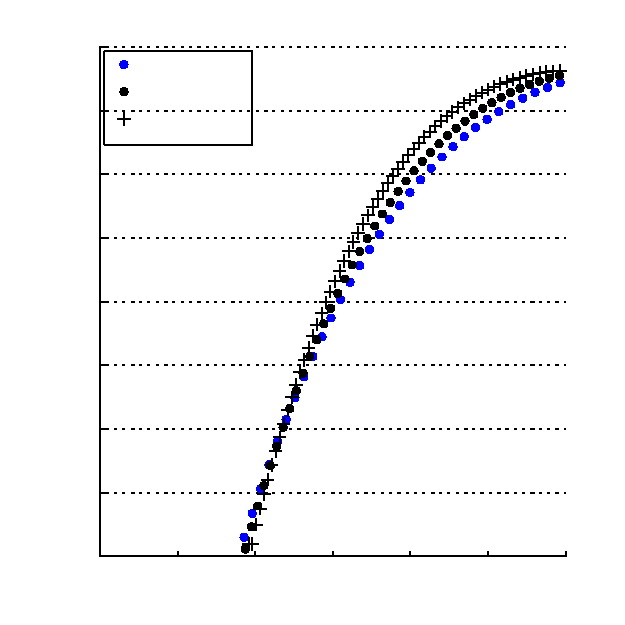
\includegraphics[width=\linewidth]{Appendix3/Figs/dtl_slope_comp_temp-inc}
\end{picture}%
\begin{picture}(300,300)(0,0)
\fontsize{8}{0}
\selectfont\put(271.496,27.9883){\makebox(0,0)[t]{\textcolor[rgb]{0,0,0}{{1}}}}
\selectfont\put(43.0039,277.492){\makebox(0,0)[r]{\textcolor[rgb]{0,0,0}{{1e-14}}}}
\selectfont\put(43.0039,246.93){\makebox(0,0)[r]{\textcolor[rgb]{0,0,0}{{1e-16}}}}
\selectfont\put(43.0039,216.371){\makebox(0,0)[r]{\textcolor[rgb]{0,0,0}{{1e-18}}}}
\selectfont\put(43.0039,185.809){\makebox(0,0)[r]{\textcolor[rgb]{0,0,0}{{1e-20}}}}
\selectfont\put(43.0039,155.246){\makebox(0,0)[r]{\textcolor[rgb]{0,0,0}{{1e-22}}}}
\selectfont\put(43.0039,124.684){\makebox(0,0)[r]{\textcolor[rgb]{0,0,0}{{1e-24}}}}
\selectfont\put(43.0039,94.1211){\makebox(0,0)[r]{\textcolor[rgb]{0,0,0}{{1e-26}}}}
\selectfont\put(43.0039,63.5625){\makebox(0,0)[r]{\textcolor[rgb]{0,0,0}{{1e-28}}}}
\selectfont\put(43.0039,33){\makebox(0,0)[r]{\textcolor[rgb]{0,0,0}{{1e-30}}}}
\selectfont\put(159.746,8.9883){\makebox(0,0)[t]{\textcolor[rgb]{0,0,0}{{Slope progression}}}}
\selectfont\put(-10.0039,155.246){\rotatebox{90}{\makebox(0,0)[b]{\textcolor[rgb]{0,0,0}{{dP(Met.)/dF [1/Hz]}}}}}
\selectfont\put(234.246,27.9883){\makebox(0,0)[t]{\textcolor[rgb]{0,0,0}{{0.95}}}}
\selectfont\put(196.996,27.9883){\makebox(0,0)[t]{\textcolor[rgb]{0,0,0}{{0.9}}}}
\selectfont\put(159.746,27.9883){\makebox(0,0)[t]{\textcolor[rgb]{0,0,0}{{0.85}}}}
\selectfont\put(122.492,27.9883){\makebox(0,0)[t]{\textcolor[rgb]{0,0,0}{{0.8}}}}
\selectfont\put(85.2422,27.9883){\makebox(0,0)[t]{\textcolor[rgb]{0,0,0}{{0.75}}}}
\selectfont\put(47.9922,27.9883){\makebox(0,0)[t]{\textcolor[rgb]{0,0,0}{{0.7}}}}
\fontsize{7}{0}
\selectfont\put(68.9961,268.992){\makebox(0,0)[l]{\textcolor[rgb]{0,0,0}{{-50\degree C}}}}
\selectfont\put(68.9961,255.992){\makebox(0,0)[l]{\textcolor[rgb]{0,0,0}{{25\degree C}}}}
\selectfont\put(68.9961,242.992){\makebox(0,0)[l]{\textcolor[rgb]{0,0,0}{{175\degree C}}}}
\end{picture}

   \subcaption{DT temperature variation}
   \label{fig:dtl_slope_temp}
 \end{subfigure}
 \caption{Derivative of the probability to generate metastability}
 \label{fig:slop_deriv_sa_dt_temp}
\end{figure}

\figurename~\ref{fig:slop_deriv_sa_dt_temp} (a) compares the topology at 25\degree C. We conclude that the topology does not impact variation of probability. 

\figurename~\ref{fig:slop_deriv_sa_dt_temp} (b) represents the variation of the probability for the double tail for three different temperatures. The temperature impacts most the corner than the slope of the rising probability.

For both comparators, the variation of probability over temperature exhibited are similar and only the value of probability change due to a SA comparator being slower than the DT one. At $25 \degree C$ and $175 \degree C$ for a clock frequency of 150 MHz, the probability to generate metastable DFFs output is less than $10^{-18}$ and $5\times 10^{-10}$ for the DT\@. For the SA the probability is $2\times 10^{-17}$ and $3\times 10^{-9}$.

Then the probability of comparators to be in a metastable state is depicted by the \figurename~\ref{fig:prob_met_temp}. Compared to previous probability, this probability rises up to 1 with the increasing clock frequency and the temperature shift the PDF to smaller clock frequencies. But it also demonstrates that transition from low to high probability is never instantaneous, and its slope does not depends on temperature. With layout respecting good-matching practices, the slope is a result of either the noise as reported in~\cite{metastability_figueiredo_2013}, or the process variation, or the repartition of $\Delta V_{in}$ as a random variable. In the results presented the noise is not taken into account.

From (\ref{eqn:error_prob_met}), those results in the absence of noise and hysteresis have an estimated error at 175\(\degree \)C of $1.6\times10^{-13}$ and $3\times10^{-13}$ respectively for the DT, \figurename~\ref{fig:DTL_prob_met_temp}, and the SA, \figurename~\ref{fig:SA_prob_met_temp}, on the probability of metastability where the probability level is $10^{-9}$.

Concerning the probability of generating metastability and to be metastable, they do not follow the same law of probability. Indeed, the PDF of generating metastability decreases for very high frequencies since delay is far much greater than the allotted time, and reach with an ever smaller probability the metastable zone of DFFs. Moreover, increasing the differential input shifts the PDF to high frequencies. Therefore, an slowly increasing top appears on the PDF\@.

\begin{figure}[htp]
	\centering
	\hspace{0.1cm}
	\begin{subfigure}[b]{0.48\textwidth}
		% Title: glps_renderer figure
% Creator: GL2PS 1.3.9, (C) 1999-2015 C. Geuzaine
% For: Octave
% CreationDate: Thu Nov 03 13:00:57 2016
\setlength{\unitlength}{0.0033\linewidth}
\begin{picture}(0,0)
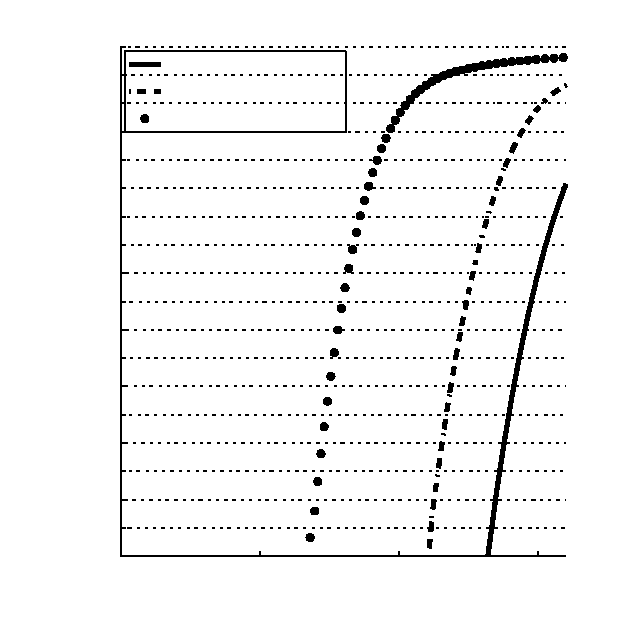
\includegraphics[width=\linewidth]{Appendix3/Figs/DTL_prob_met_temp-inc}
\end{picture}%
\begin{picture}(300,300)(0,0)
\fontsize{8}{0}
\selectfont\put(0.0039,155.246){\rotatebox{90}{\makebox(0,0)[b]{\textcolor[rgb]{0,0,0}{{P(Met.)}}}}}
\selectfont\put(164.746,6.9883){\makebox(0,0)[t]{\textcolor[rgb]{0,0,0}{{Frequency [MHz]}}}}
\selectfont\put(53.0039,277.492){\makebox(0,0)[r]{\textcolor[rgb]{0,0,0}{{1}}}}
%\selectfont\put(53.0039,263.91){\makebox(0,0)[r]{\textcolor[rgb]{0,0,0}{{1e-01}}}}
\selectfont\put(53.0039,250.328){\makebox(0,0)[r]{\textcolor[rgb]{0,0,0}{{1e-02}}}}
%\selectfont\put(53.0039,236.742){\makebox(0,0)[r]{\textcolor[rgb]{0,0,0}{{1e-03}}}}
\selectfont\put(53.0039,223.16){\makebox(0,0)[r]{\textcolor[rgb]{0,0,0}{{1e-04}}}}
%\selectfont\put(53.0039,209.578){\makebox(0,0)[r]{\textcolor[rgb]{0,0,0}{{1e-05}}}}
\selectfont\put(53.0039,195.996){\makebox(0,0)[r]{\textcolor[rgb]{0,0,0}{{1e-06}}}}
%\selectfont\put(53.0039,182.41){\makebox(0,0)[r]{\textcolor[rgb]{0,0,0}{{1e-07}}}}
\selectfont\put(53.0039,168.828){\makebox(0,0)[r]{\textcolor[rgb]{0,0,0}{{1e-08}}}}
%\selectfont\put(53.0039,155.246){\makebox(0,0)[r]{\textcolor[rgb]{0,0,0}{{1e-09}}}}
\selectfont\put(53.0039,141.664){\makebox(0,0)[r]{\textcolor[rgb]{0,0,0}{{1e-10}}}}
%\selectfont\put(53.0039,128.078){\makebox(0,0)[r]{\textcolor[rgb]{0,0,0}{{1e-11}}}}
\selectfont\put(53.0039,114.496){\makebox(0,0)[r]{\textcolor[rgb]{0,0,0}{{1e-12}}}}
%\selectfont\put(53.0039,100.914){\makebox(0,0)[r]{\textcolor[rgb]{0,0,0}{{1e-13}}}}
\selectfont\put(53.0039,87.332){\makebox(0,0)[r]{\textcolor[rgb]{0,0,0}{{1e-14}}}}
%\selectfont\put(53.0039,73.75){\makebox(0,0)[r]{\textcolor[rgb]{0,0,0}{{1e-15}}}}
\selectfont\put(53.0039,60.1641){\makebox(0,0)[r]{\textcolor[rgb]{0,0,0}{{1e-16}}}}
%\selectfont\put(53.0039,46.582){\makebox(0,0)[r]{\textcolor[rgb]{0,0,0}{{1e-17}}}}
\selectfont\put(53.0039,33){\makebox(0,0)[r]{\textcolor[rgb]{0,0,0}{{1e-18}}}}
\selectfont\put(258.152,27.9883){\makebox(0,0)[t]{\textcolor[rgb]{0,0,0}{{200}}}}
\selectfont\put(191.434,27.9883){\makebox(0,0)[t]{\textcolor[rgb]{0,0,0}{{150}}}}
\selectfont\put(124.711,27.9883){\makebox(0,0)[t]{\textcolor[rgb]{0,0,0}{{100}}}}
\fontsize{7}{0}
\selectfont\put(78.9961,270.992){\makebox(0,0)[l]{\textcolor[rgb]{0,0,0}{{$-50 \degree C$}}}}
\selectfont\put(78.9961,257.992){\makebox(0,0)[l]{\textcolor[rgb]{0,0,0}{{$+25 \degree C$}}}}
\selectfont\put(78.9961,245.992){\makebox(0,0)[l]{\textcolor[rgb]{0,0,0}{{$+175 \degree C$}}}}
\fontsize{8}{0}
\selectfont\put(57.9922,27.9883){\makebox(0,0)[t]{\textcolor[rgb]{0,0,0}{{50}}}}
\end{picture}

		\subcaption{Double Tail}
		\label{fig:DTL_prob_met_temp}
	\end{subfigure}
	\hspace{0.1cm}
	\begin{subfigure}[b]{0.48\textwidth}
		% Title: glps_renderer figure
% Creator: GL2PS 1.3.9, (C) 1999-2015 C. Geuzaine
% For: Octave
% CreationDate: Fri Oct 28 13:36:37 2016
\setlength{\unitlength}{0.0033\linewidth}
\begin{picture}(0,0)
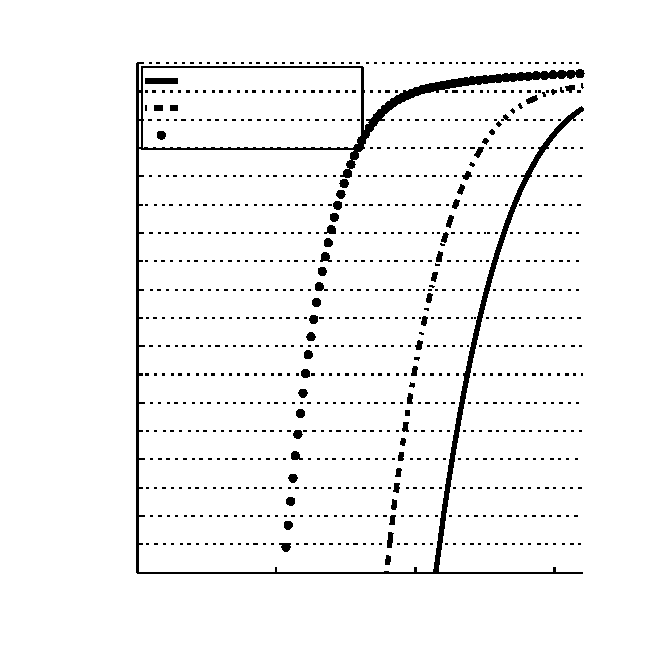
\includegraphics[width=\linewidth]{Appendix3/Figs/SA_prob_met_temp-inc}
\end{picture}%
\begin{picture}(300,300)(0,0)
\fontsize{8}{0}
\selectfont\put(0.0039,155.246){\rotatebox{90}{\makebox(0,0)[b]{\textcolor[rgb]{0,0,0}{{P(Met.)}}}}}
\selectfont\put(164.746,6.9883){\makebox(0,0)[t]{\textcolor[rgb]{0,0,0}{{Frequency [MHz]}}}}
\selectfont\put(53.0039,277.492){\makebox(0,0)[r]{\textcolor[rgb]{0,0,0}{{1}}}}
%\selectfont\put(53.0039,263.91){\makebox(0,0)[r]{\textcolor[rgb]{0,0,0}{{1e-01}}}}
\selectfont\put(53.0039,250.328){\makebox(0,0)[r]{\textcolor[rgb]{0,0,0}{{1e-02}}}}
%\selectfont\put(53.0039,236.742){\makebox(0,0)[r]{\textcolor[rgb]{0,0,0}{{1e-03}}}}
\selectfont\put(53.0039,223.16){\makebox(0,0)[r]{\textcolor[rgb]{0,0,0}{{1e-04}}}}
%\selectfont\put(53.0039,209.578){\makebox(0,0)[r]{\textcolor[rgb]{0,0,0}{{1e-05}}}}
\selectfont\put(53.0039,195.996){\makebox(0,0)[r]{\textcolor[rgb]{0,0,0}{{1e-06}}}}
%\selectfont\put(53.0039,182.41){\makebox(0,0)[r]{\textcolor[rgb]{0,0,0}{{1e-07}}}}
\selectfont\put(53.0039,168.828){\makebox(0,0)[r]{\textcolor[rgb]{0,0,0}{{1e-08}}}}
%\selectfont\put(53.0039,155.246){\makebox(0,0)[r]{\textcolor[rgb]{0,0,0}{{1e-09}}}}
\selectfont\put(53.0039,141.664){\makebox(0,0)[r]{\textcolor[rgb]{0,0,0}{{1e-10}}}}
%\selectfont\put(53.0039,128.078){\makebox(0,0)[r]{\textcolor[rgb]{0,0,0}{{1e-11}}}}
\selectfont\put(53.0039,114.496){\makebox(0,0)[r]{\textcolor[rgb]{0,0,0}{{1e-12}}}}
%\selectfont\put(53.0039,100.914){\makebox(0,0)[r]{\textcolor[rgb]{0,0,0}{{1e-13}}}}
\selectfont\put(53.0039,87.332){\makebox(0,0)[r]{\textcolor[rgb]{0,0,0}{{1e-14}}}}
%\selectfont\put(53.0039,73.75){\makebox(0,0)[r]{\textcolor[rgb]{0,0,0}{{1e-15}}}}
\selectfont\put(53.0039,60.1641){\makebox(0,0)[r]{\textcolor[rgb]{0,0,0}{{1e-16}}}}
%\selectfont\put(53.0039,46.582){\makebox(0,0)[r]{\textcolor[rgb]{0,0,0}{{1e-17}}}}
\selectfont\put(53.0039,33){\makebox(0,0)[r]{\textcolor[rgb]{0,0,0}{{1e-18}}}}
\selectfont\put(258.152,27.9883){\makebox(0,0)[t]{\textcolor[rgb]{0,0,0}{{200}}}}
\selectfont\put(191.434,27.9883){\makebox(0,0)[t]{\textcolor[rgb]{0,0,0}{{150}}}}
\selectfont\put(124.711,27.9883){\makebox(0,0)[t]{\textcolor[rgb]{0,0,0}{{100}}}}
\fontsize{7}{0}
\selectfont\put(78.9961,270.992){\makebox(0,0)[l]{\textcolor[rgb]{0,0,0}{{$-50 \degree C$}}}}
\selectfont\put(78.9961,257.992){\makebox(0,0)[l]{\textcolor[rgb]{0,0,0}{{$+25 \degree C$}}}}
\selectfont\put(78.9961,245.992){\makebox(0,0)[l]{\textcolor[rgb]{0,0,0}{{$+175 \degree C$}}}}
\fontsize{8}{0}
\selectfont\put(57.9922,27.9883){\makebox(0,0)[t]{\textcolor[rgb]{0,0,0}{{50}}}}
\end{picture}

		\subcaption{Strong ARM}
		\label{fig:SA_prob_met_temp}
	\end{subfigure}
	\caption{P(Metastability) of latches for -50$\degree C$, +25$\degree C$, +175$\degree C$, $\Delta V_{in} \in \pm 450 mV$}
	\label{fig:prob_met_temp}
\end{figure}

%Figure \ref{fig:sa_prob_temp_freq_matlab} and \ref{fig:dtl_prob_temp_freq_matlab} depicts the probability of metastability for a $\Delta V_{in}$ from 100 $\mu V$ to 450 mV, a temperature range from -50\degree C to +175\degree C at different clock frequency. The duty cycle of clock is to 50 \%.

%\begin{figure}[!ht]
%	\centering
%	\begin{minipage}[b]{0.48\linewidth}
%		% Title: glps_renderer figure
% Creator: GL2PS 1.3.9, (C) 1999-2015 C. Geuzaine
% For: Octave
% CreationDate: Fri Oct 07 16:41:29 2016
\setlength{\unitlength}{0.005\linewidth}
\begin{picture}(0,0)
\includegraphics[width=\linewidth]{./SA_xt018_prob_temp_freq_matlab-inc}
\end{picture}%
\begin{picture}(200,150)(0,0)
\fontsize{8}{0}
\selectfont\put(97.4727,7){\makebox(0,0)[t]{\textcolor[rgb]{0,0,0}{{FREQUENCY [MHz]}}}}
\selectfont\put(36.7734,126.324){\makebox(0,0)[r]{\textcolor[rgb]{0,0,0}{{150}}}}
\selectfont\put(36.7734,101.492){\makebox(0,0)[r]{\textcolor[rgb]{0,0,0}{{100}}}}
\selectfont\put(36.7734,76.6563){\makebox(0,0)[r]{\textcolor[rgb]{0,0,0}{{50}}}}
\selectfont\put(36.7734,51.8203){\makebox(0,0)[r]{\textcolor[rgb]{0,0,0}{{0}}}}
\selectfont\put(36.7734,26.9883){\makebox(0,0)[r]{\textcolor[rgb]{0,0,0}{{-50}}}}
\selectfont\put(119.746,21.9961){\makebox(0,0)[t]{\textcolor[rgb]{0,0,0}{{200}}}}
\selectfont\put(86.3359,21.9961){\makebox(0,0)[t]{\textcolor[rgb]{0,0,0}{{150}}}}
\selectfont\put(52.9258,21.9961){\makebox(0,0)[t]{\textcolor[rgb]{0,0,0}{{100}}}}
\selectfont\put(14.7734,72.8633){\rotatebox{90}{\makebox(0,0)[b]{\textcolor[rgb]{0,0,0}{{TEMPERATURE [$^\circ$C]}}}}}
\selectfont\put(180.648,36.4258){\makebox(0,0)[l]{\textcolor[rgb]{0,0,0}{{1}}}}
\selectfont\put(180.648,58.2773){\makebox(0,0)[l]{\textcolor[rgb]{0,0,0}{{2}}}}
\selectfont\put(180.648,80.1328){\makebox(0,0)[l]{\textcolor[rgb]{0,0,0}{{3}}}}
\selectfont\put(180.648,101.988){\makebox(0,0)[l]{\textcolor[rgb]{0,0,0}{{4}}}}
\selectfont\put(180.648,123.844){\makebox(0,0)[l]{\textcolor[rgb]{0,0,0}{{5}}}}
\end{picture}

%		\subcaption{Strong-Arm}
%		\label{fig:sa_prob_temp_freq_matlab}
%	\end{minipage}
%	\begin{minipage}[b]{0.48\linewidth}
%		% Title: glps_renderer figure
% Creator: GL2PS 1.3.9, (C) 1999-2015 C. Geuzaine
% For: Octave
% CreationDate: Fri Oct 07 16:42:10 2016
\setlength{\unitlength}{0.005\linewidth}
\begin{picture}(0,0)
\includegraphics[width=\linewidth]{./DTL_xt018_prob_temp_freq_matlab-inc}
\end{picture}%
\begin{picture}(200,150)(0,0)
\fontsize{8}{0}
\selectfont\put(97.4727,7){\makebox(0,0)[t]{\textcolor[rgb]{0,0,0}{{FREQUENCY [MHz]}}}}
\selectfont\put(36.7734,126.324){\makebox(0,0)[r]{\textcolor[rgb]{0,0,0}{{150}}}}
\selectfont\put(36.7734,101.492){\makebox(0,0)[r]{\textcolor[rgb]{0,0,0}{{100}}}}
\selectfont\put(36.7734,76.6563){\makebox(0,0)[r]{\textcolor[rgb]{0,0,0}{{50}}}}
\selectfont\put(36.7734,51.8203){\makebox(0,0)[r]{\textcolor[rgb]{0,0,0}{{0}}}}
\selectfont\put(36.7734,26.9883){\makebox(0,0)[r]{\textcolor[rgb]{0,0,0}{{-50}}}}
\selectfont\put(119.746,21.9961){\makebox(0,0)[t]{\textcolor[rgb]{0,0,0}{{200}}}}
\selectfont\put(86.3359,21.9961){\makebox(0,0)[t]{\textcolor[rgb]{0,0,0}{{150}}}}
\selectfont\put(52.9258,21.9961){\makebox(0,0)[t]{\textcolor[rgb]{0,0,0}{{100}}}}
\selectfont\put(14.7734,72.8633){\rotatebox{90}{\makebox(0,0)[b]{\textcolor[rgb]{0,0,0}{{TEMPERATURE [$^\circ$C]}}}}}
\selectfont\put(180.648,35.4102){\makebox(0,0)[l]{\textcolor[rgb]{0,0,0}{{1}}}}
\selectfont\put(180.648,56.2539){\makebox(0,0)[l]{\textcolor[rgb]{0,0,0}{{2}}}}
\selectfont\put(180.648,77.0977){\makebox(0,0)[l]{\textcolor[rgb]{0,0,0}{{3}}}}
\selectfont\put(180.648,97.9375){\makebox(0,0)[l]{\textcolor[rgb]{0,0,0}{{4}}}}
\selectfont\put(180.648,118.781){\makebox(0,0)[l]{\textcolor[rgb]{0,0,0}{{5}}}}
\end{picture}

%		\subcaption{Double tail}
%		\label{fig:dtl_prob_temp_freq_matlab}
%	\end{minipage}
%	\caption{Estimation of the metastability probability percentage over the temperature and process at different the clock frequencies}
%\end{figure}

% as depicted in Figure \ref{fig:prob_pdfs}.

%\begin{figure}[!ht]
%	\centering
%	\begin{minipage}[t]{0.43\linewidth}
%		% Title: glps_renderer figure
% Creator: GL2PS 1.3.9, (C) 1999-2015 C. Geuzaine
% For: Octave
% CreationDate: Fri Oct 28 15:58:21 2016
\setlength{\unitlength}{0.0033\linewidth}
\begin{picture}(0,0)
\includegraphics[width=\linewidth]{Appendix3/Figs/DTL_prob_met_zone_temp-pdf}
\end{picture}%
\begin{picture}(300,300)(0,0)
\fontsize{7}{0}
\selectfont\put(0.0039,155.246){\rotatebox{90}{\makebox(0,0)[b]{\textcolor[rgb]{0,0,0}{{P(Met. Zone)}}}}}
\selectfont\put(162.746,10.0078){\makebox(0,0)[t]{\textcolor[rgb]{0,0,0}{{Frequency [MHz]}}}}
\selectfont\put(49.0039,277.492){\makebox(0,0)[r]{\textcolor[rgb]{0,0,0}{{1e-04}}}}
%\selectfont\put(49.0039,260.027){\makebox(0,0)[r]{\textcolor[rgb]{0,0,0}{{1e-05}}}}
\selectfont\put(49.0039,242.566){\makebox(0,0)[r]{\textcolor[rgb]{0,0,0}{{1e-06}}}}
%\selectfont\put(49.0039,225.102){\makebox(0,0)[r]{\textcolor[rgb]{0,0,0}{{1e-07}}}}
\selectfont\put(49.0039,207.637){\makebox(0,0)[r]{\textcolor[rgb]{0,0,0}{{1e-08}}}}
%\selectfont\put(49.0039,190.172){\makebox(0,0)[r]{\textcolor[rgb]{0,0,0}{{1e-09}}}}
\selectfont\put(49.0039,172.711){\makebox(0,0)[r]{\textcolor[rgb]{0,0,0}{{1e-10}}}}
%\selectfont\put(49.0039,155.246){\makebox(0,0)[r]{\textcolor[rgb]{0,0,0}{{1e-11}}}}
\selectfont\put(49.0039,137.781){\makebox(0,0)[r]{\textcolor[rgb]{0,0,0}{{1e-12}}}}
%\selectfont\put(49.0039,120.316){\makebox(0,0)[r]{\textcolor[rgb]{0,0,0}{{1e-13}}}}
\selectfont\put(49.0039,102.855){\makebox(0,0)[r]{\textcolor[rgb]{0,0,0}{{1e-14}}}}
%\selectfont\put(49.0039,85.3906){\makebox(0,0)[r]{\textcolor[rgb]{0,0,0}{{1e-15}}}}
\selectfont\put(49.0039,67.9258){\makebox(0,0)[r]{\textcolor[rgb]{0,0,0}{{1e-16}}}}
%\selectfont\put(49.0039,50.4648){\makebox(0,0)[r]{\textcolor[rgb]{0,0,0}{{1e-17}}}}
\selectfont\put(49.0039,33){\makebox(0,0)[r]{\textcolor[rgb]{0,0,0}{{1e-18}}}}
\selectfont\put(269.621,28.0078){\makebox(0,0)[t]{\textcolor[rgb]{0,0,0}{{1200}}}}
\selectfont\put(232.121,28.0078){\makebox(0,0)[t]{\textcolor[rgb]{0,0,0}{{1000}}}}
\selectfont\put(194.621,28.0078){\makebox(0,0)[t]{\textcolor[rgb]{0,0,0}{{800}}}}
\selectfont\put(157.117,28.0078){\makebox(0,0)[t]{\textcolor[rgb]{0,0,0}{{600}}}}
\selectfont\put(119.617,28.0078){\makebox(0,0)[t]{\textcolor[rgb]{0,0,0}{{400}}}}
\fontsize{5}{0}
\selectfont\put(202.496,268.992){\makebox(0,0)[l]{\textcolor[rgb]{0,0,0}{{$-50 \degree C$}}}}
\selectfont\put(202.496,255.992){\makebox(0,0)[l]{\textcolor[rgb]{0,0,0}{{$+25 \degree C$}}}}
\selectfont\put(202.496,242.992){\makebox(0,0)[l]{\textcolor[rgb]{0,0,0}{{$+175 \degree C$}}}}
\fontsize{7}{0}
\selectfont\put(82.1172,28.0078){\makebox(0,0)[t]{\textcolor[rgb]{0,0,0}{{200}}}}
\end{picture}

%		\subcaption{$P(Metastability)$ of DFFs}
%		\label{fig:DTL_prob_met_zone_temp-pdf}
%	\end{minipage}
%	\hspace{0.1cm}
%	\begin{minipage}[t]{0.43\linewidth}
%		% Title: glps_renderer figure
% Creator: GL2PS 1.3.9, (C) 1999-2015 C. Geuzaine
% For: Octave
% CreationDate: Fri Oct 28 15:58:21 2016
\setlength{\unitlength}{0.0033\linewidth}
\begin{picture}(0,0)
\includegraphics[width=\linewidth]{Appendix3/Figs/DTL_prob_met_temp-pdf}
\end{picture}%
\begin{picture}(300,300)(0,0)
\fontsize{7}{0}
\selectfont\put(0.0039,155.246){\rotatebox{90}{\makebox(0,0)[b]{\textcolor[rgb]{0,0,0}{{P(Met.)}}}}}
\selectfont\put(164.746,10.9883){\makebox(0,0)[t]{\textcolor[rgb]{0,0,0}{{Frequency [MHz]}}}}
\selectfont\put(53.0039,277.492){\makebox(0,0)[r]{\textcolor[rgb]{0,0,0}{{1}}}}
%\selectfont\put(53.0039,263.91){\makebox(0,0)[r]{\textcolor[rgb]{0,0,0}{{1e-01}}}}
\selectfont\put(53.0039,250.328){\makebox(0,0)[r]{\textcolor[rgb]{0,0,0}{{1e-02}}}}
%\selectfont\put(53.0039,236.742){\makebox(0,0)[r]{\textcolor[rgb]{0,0,0}{{1e-03}}}}
\selectfont\put(53.0039,223.16){\makebox(0,0)[r]{\textcolor[rgb]{0,0,0}{{1e-04}}}}
%\selectfont\put(53.0039,209.578){\makebox(0,0)[r]{\textcolor[rgb]{0,0,0}{{1e-05}}}}
\selectfont\put(53.0039,195.996){\makebox(0,0)[r]{\textcolor[rgb]{0,0,0}{{1e-06}}}}
%\selectfont\put(53.0039,182.41){\makebox(0,0)[r]{\textcolor[rgb]{0,0,0}{{1e-07}}}}
\selectfont\put(53.0039,168.828){\makebox(0,0)[r]{\textcolor[rgb]{0,0,0}{{1e-08}}}}
%\selectfont\put(53.0039,155.246){\makebox(0,0)[r]{\textcolor[rgb]{0,0,0}{{1e-09}}}}
\selectfont\put(53.0039,141.664){\makebox(0,0)[r]{\textcolor[rgb]{0,0,0}{{1e-10}}}}
%\selectfont\put(53.0039,128.078){\makebox(0,0)[r]{\textcolor[rgb]{0,0,0}{{1e-11}}}}
\selectfont\put(53.0039,114.496){\makebox(0,0)[r]{\textcolor[rgb]{0,0,0}{{1e-12}}}}
%\selectfont\put(53.0039,100.914){\makebox(0,0)[r]{\textcolor[rgb]{0,0,0}{{1e-13}}}}
\selectfont\put(53.0039,87.332){\makebox(0,0)[r]{\textcolor[rgb]{0,0,0}{{1e-14}}}}
%\selectfont\put(53.0039,73.75){\makebox(0,0)[r]{\textcolor[rgb]{0,0,0}{{1e-15}}}}
\selectfont\put(53.0039,60.1641){\makebox(0,0)[r]{\textcolor[rgb]{0,0,0}{{1e-16}}}}
%\selectfont\put(53.0039,46.582){\makebox(0,0)[r]{\textcolor[rgb]{0,0,0}{{1e-17}}}}
\selectfont\put(53.0039,33){\makebox(0,0)[r]{\textcolor[rgb]{0,0,0}{{1e-18}}}}
\selectfont\put(269.656,27.9883){\makebox(0,0)[t]{\textcolor[rgb]{0,0,0}{{1200}}}}
\selectfont\put(232.844,27.9883){\makebox(0,0)[t]{\textcolor[rgb]{0,0,0}{{1000}}}}
\selectfont\put(196.035,27.9883){\makebox(0,0)[t]{\textcolor[rgb]{0,0,0}{{800}}}}
\selectfont\put(159.223,27.9883){\makebox(0,0)[t]{\textcolor[rgb]{0,0,0}{{600}}}}
\selectfont\put(122.41,27.9883){\makebox(0,0)[t]{\textcolor[rgb]{0,0,0}{{400}}}}
\fontsize{5}{0}
\selectfont\put(202.496,168.246){\makebox(0,0)[l]{\textcolor[rgb]{0,0,0}{{$-50 \degree C$}}}}
\selectfont\put(202.496,155.246){\makebox(0,0)[l]{\textcolor[rgb]{0,0,0}{{$+25 \degree C$}}}}
\selectfont\put(202.496,142.246){\makebox(0,0)[l]{\textcolor[rgb]{0,0,0}{{$+175 \degree C$}}}}
\fontsize{7}{0}
\selectfont\put(85.6016,27.9883){\makebox(0,0)[t]{\textcolor[rgb]{0,0,0}{{200}}}}
\end{picture}

%		\subcaption{$P(Metastability)$ of the DT}
%		\label{fig:DTL_prob_met_temp-pdf}
%	\end{minipage}
%	\caption{PDF comparison based on Double-Tail simulation results over temperature, $\Delta V_{in} \in [-450, +450] mV$}
%	\label{fig:prob_pdfs}
%\end{figure}


 
%  between 180 MHz and 490 MHz. To the contrary the PDF of being metastable tends to 1 for an increasing clock frequency since comparators do not respond in time.
 
 %For the Figure \ref{fig:DTL_prob_met_zone_temp-pdf},
% The spread around the peak of probability over temperature is decreasing as far the temperature is increasing by $T_{clk}/2\tau$ for an equi-level of probability in both topologies over the temperature range. This is explained by a lesser current variation due to the differential input voltages applied on the differential pair transistors with the temperature.